\documentclass[11pt,fleqn]{exam}
\usepackage[utf8]{inputenc}

\usepackage[margin=1in]{geometry}
\usepackage{amsmath,amssymb}
\usepackage{gensymb}
\usepackage{multicol}
\usepackage{float}
\usepackage{graphicx}
\usepackage{units,icomma}
\usepackage[bahasa]{babel}
\usepackage[colorlinks,linkcolor=blue,urlcolor=blue]{hyperref}
\usepackage[margin=1.5cm]{caption}
\usepackage{wasysym}
\usepackage{tikzsymbols}
\usepackage[shortlabels]{enumitem}

\hyphenation{
  chro-no-ampe-ro-met-ric
  ber-dia-me-ter
  de-ngan
  meng-alam-i
  me-nem-pati
  mic-ro-graphs
  man-hat-tan-henge}

\addto\extrasbahasa{
	\def\figureautorefname{Gambar}
}

\renewcommand{\figurename}{Gambar.}
\def\equationautorefname{Persamaan}
\newcommand{\class}{OLIMPIADE ASTRONOMI}
\newcommand{\term}{Tingkat Provinsi - 2019}
\newcommand{\examnum}{OSP Astronomi 2019}
%\newcommand{\examdate}{11/02/2014}
%\newcommand{\timelimit}{120 Minutes}

%%%%%%%%% Units and Symbols
\newcommand*{\kms}{km s\ensuremath{^{-1}}}
\newcommand*{\Msun}{\ensuremath{M_{\odot}}}
\newcommand*{\Lsun}{\ensuremath{L_{\odot}}}
\newcommand*{\Rsun}{\ensuremath{R_{\odot}}}
\newcommand*{\Mstar}{\ensuremath{M_{\star}}}
\newcommand*{\Lstar}{\ensuremath{L_{\star}}}
\newcommand*{\Rstar}{\ensuremath{R_{\star}}}

\newcommand*{\jam}{\ensuremath{^{j}}}
\newcommand*{\h}{\ensuremath{^{h}}}
\newcommand*{\m}{\ensuremath{^{m}}}
\newcommand*{\s}{\ensuremath{^{s}}}
\newcommand*{\de}{\ensuremath{^{\circ}}}
\newcommand*{\am}{'}
\newcommand*{\as}{''}

\newcommand*{\alp}{\ensuremath{\alpha}}
\newcommand*{\del}{\ensuremath{\delta}}


\pagestyle{head}
\firstpageheader{}{}{}
\runningheader{\examnum}{}{Halaman \thepage\ dari \numpages}
\runningheadrule


\begin{document}

\noindent
\begin{tabular*}{\textwidth}{l @{\extracolsep{\fill}} r @{\extracolsep{6pt}} l}
\textbf{\class} \\% & \textbf{Name:} & \makebox[2in]{\hrulefill}\\
\textbf{\term}  %&&\\
%\textbf{\examnum} &&\\
%\textbf{\examdate} &&\\
%\textbf{Time Limit: \timelimit} & Teaching Assistant & \makebox[2in]{\hrulefill}
\end{tabular*}\\
\rule[2ex]{\textwidth}{2pt}

\noindent
\begin{tabular}{ll}
Copyright (c) 2019 & Ridlo W. Wibowo (ridlo.w.wibowo@gmail.com)\\
                   & Sulistiyowati (sulis.astro08@gmail.com)
\end{tabular}

\vspace{0.3cm}
\noindent
Solusi ini dibuat tanpa jaminan kesesuaian dengan solusi resmi dari juri olimpiade sains bidang Astronomi. Pengguna boleh menyebarluaskan dan/atau memodifikasi solusi ini dengan mencantumkan sumber asli. Hak cipta soal ada pada Kemendiknas dan dilindungi undang-undang. Jika ada kesalahan jawaban/penulisan harap melaporkan ke alamat surel di atas.

\vspace{0.4cm}
\noindent
\rule[2ex]{\textwidth}{1.5pt}

\textbf{Soal Pilihan Ganda dan Benar Salah}

\begin{questions}

\question Claudius Ptolomeus adalah seorang ilmuwan Yunani yang mengajukan model alam semesta yang dikenal dengan model Geosentris. Dari pernyataan berikut ini, pilihlah jawaban yang SALAH menurut model Ptolomeus
\begin{choices}
\choice Bintang-bintang tidak bergerak
\choice Bumi tidak berada di pusat orbit lingkaran planet
\choice Untuk menjelaskan gerak berbalik planet (\textit{retrograde motion}), ditambahkan lingkaran-lingkaran kecil pada setiap orbit planet
\choice Bumi dianggap diam
\choice Planet bergerak dengan laju tetap
\end{choices}


\textit{Jawaban: } mungkin A atau B

Pilihan A. Apa maksud ``tidak bergerak'' di sini? Apakah maksudnya relatif terhadap mereka sendiri (tidak punya gerak diri)? Menurut model Ptolomeus bintang seperti menempel (tidak bergerak) di bola langit, kemudian bola langit ini berputar (bergerak) mengitari Bumi. 

Pilihan B. ``Seberapa pusat''?

Menurut model geosentris sebelumnya, hingga saat masa Ptolomeus, Bumi merupakan pusat dari Tata Surya (dan alam semesta) dan letaknya tepat di tengah. Ptolomeus membuat sistem baru yang menempatkan Bumi tidak di pusat orbit planet, membuat titik baru bernama \textit{equant} untuk dapat menjelaskan gerak planet dengan lebih presisi. Saat itu model Ptolomeus adalah yang paling dikenal.
\begin{multicols}{2}
		\begin{figure}[H]
			\centering
			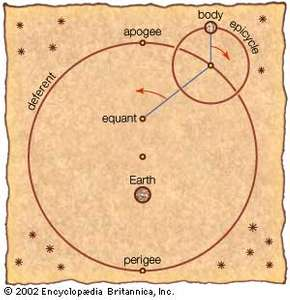
\includegraphics[width=0.3\textwidth]{ptolemic.jpg}
		\end{figure}
Setelah masa Ptolomeus, kritik terhadap model ini bermunculan. Muncul pula model-model geosentris lain, seperti model Tychonic, Arzachel (Ibn Zarqala, koreksi elips untuk Merkurius di astrolabe). Banyak astronom muslim ketika itu mulai mempertanyakan kebenaran model geosentris itu sendiri. Pada era Ibn al-Shatir mereka mulai mencoba meninggalkan model geosentris.
\end{multicols}




\vspace{0.5cm}
\question Diketahui lebar garis emisi pada panjang gelombang 6678 \AA{} pada spektrum lampu pembanding adalah 2,5 \AA. \textit{Frequency bandwidth} atau lebar garis dalam satuan frekuensi (Hz) adalah
\begin{choices}
\choice $1,1 \times 10^5$
\choice $1,6 \times 10^{11}$
\choice $4,4 \times 10^{15}$
\choice $1,2 \times 10^{18}$
\choice $1,6 \times 10^{18}$
\end{choices}


\textit{Jawaban: }B

Hubungan frekuensi ($f$) dan panjang gelombang ($\lambda$) pada cahaya (gelombang elektromagnetik) adalah
$$\lambda \cdot f = c$$
dengan $c$ adalah kecepatan cahaya.

Lebar garis dalam satuan frekuensi dapat dicari dengan cara:
\begin{eqnarray*}
\lambda_1 &=& (6678 - 1,25) \times 10^{-10} \longrightarrow f_1 = 4,4900956 \times 10^{14} \\
\lambda_2 &=& (6678 + 1,25) \times 10^{-10} \longrightarrow f_2 = 4,488415 \times 10^{14} \\
\Delta f &=& f_1 - f_2 = 1,6806137 \times 10^{11} \quad \text{Hz}
\end{eqnarray*}

\textit{Catatan}:\\
Rumus cepat, tapi hanya berlaku jika $\Delta \lambda \text{  atau  } \Delta f \lll$ 
\begin{equation*}
df = -\frac{c}{\lambda^{2}} d\lambda \qquad \text{atau} \qquad d\lambda = -\frac{c}{f^{2}} df
\end{equation*}


\vspace{0.5cm}
\question Bintang bertipe spektrum F0V memiliki magnitudo mutlak visual +2,6 dan warna intrinsik $(B-V)_0 = +0,3$. Bintang X yang bertipe spektrum F0V diamati memiliki magnitudo visual +6,79 dan $(B - V) = +0,35$. Dari informasi ini, maka jarak bintang yang diamati tersebut adalah
\begin{choices}
\choice 81,28 pc
\choice 74,13 pc
\choice 70,14 pc
\choice 68,86 pc
\choice 63,97 pc
\end{choices}


\textit{Jawaban: }E

Hubungan modulus jarak dengan melibatkan ekstingsi akibat materi antar bintang dapat dituliskan sebagai berikut:
$$V - M_{\text{v}} = -5 + 5\log{d} + A_{\text{v}}$$
dengan 
$$A_\text{v} = R \cdot E_{BV}$$
dan 
$$E_{BV} = (B - V) - (B_0 - V_0).$$

Jika kita gunakan konstanta penyerapan materi antar bintang rata-rata di bidang galaksi Bima Sakti  $R \approx 3,2$ dapat kita peroleh $A_\text{v} = R \cdot E_{BV} = 3,2 \cdot 0,05 = 0,16$. 

Jarak bintang kemudian dapat dihitung,
$$d = 10^{\frac{V - M_{\text{v}} - A_{\text{v}} + 5}{5}} = 63,97 \quad \text{pc}$$


\vspace{0.5cm}
\question Sebuah bintang berada pada tahap akhir evolusinya, yaitu pada fase pembakaran unsur berat di pusatnya. Massa dan kerapatan massa rata-rata pusat bintang masing-masing adalah 1,4 \Msun{} dan $10^{12}$ kg/m$^3$. Diketahui pusat bintang yang mengandung inti besi lembam ini runtuh menjadi pusat yang beradius 10 km. Energi total (dalam satuan Joule) yang akan dilepaskan dari suatu ledakan supernova yang berasal dari perubahan energi potensial gravitasi adalah dalam orde
\begin{choices}
\item $10^{44}$
\item $10^{46}$
\item $10^{48}$
\item $10^{50}$
\item $10^{52}$
\end{choices}


\textit{Jawaban: }B

Radius inti bintang sebelum runtuh dapat dicari terlebih dahulu,
\begin{eqnarray*}
V = \frac{M}{\rho} = 2,784 \times 10^{18} \text{  m}^3 \longrightarrow R_i &=& \sqrt[3]{\frac{3V}{4 \pi}}\\
R_i &=& 872676,37 \quad \text{meter} 
\end{eqnarray*}

Perubahan energi potensial gravitasi dapat dicari dengan asumsi inti bintang sebagai bola dengan kerapatan konstan dari pusat ke permukaannya,
\begin{eqnarray*}
\Delta E_p &=& \frac{3}{5}\frac{GM^2}{R_f} - \frac{3}{5}\frac{GM^2}{R_i}\\
\Delta E_p &=& 3 \times 10^{46} \quad \text{Joule}
\end{eqnarray*}


\vspace{0.5cm}
\question Diagram H-R dengan Matahari direpresentasikan oleh simbol bintang hitam. \textit{Panel kiri}: sumbu mendatar adalah temperatur dalam satuan Kelvin, dan sumbu tegak adalah luminositas dalam satuan \Lsun. \textit{Panel kanan}: sumbu mendatar adalah kelas spektrum, dan sumbu tegak adalah magnitudo mutlak. 
\begin{figure}[H]
	\centering
	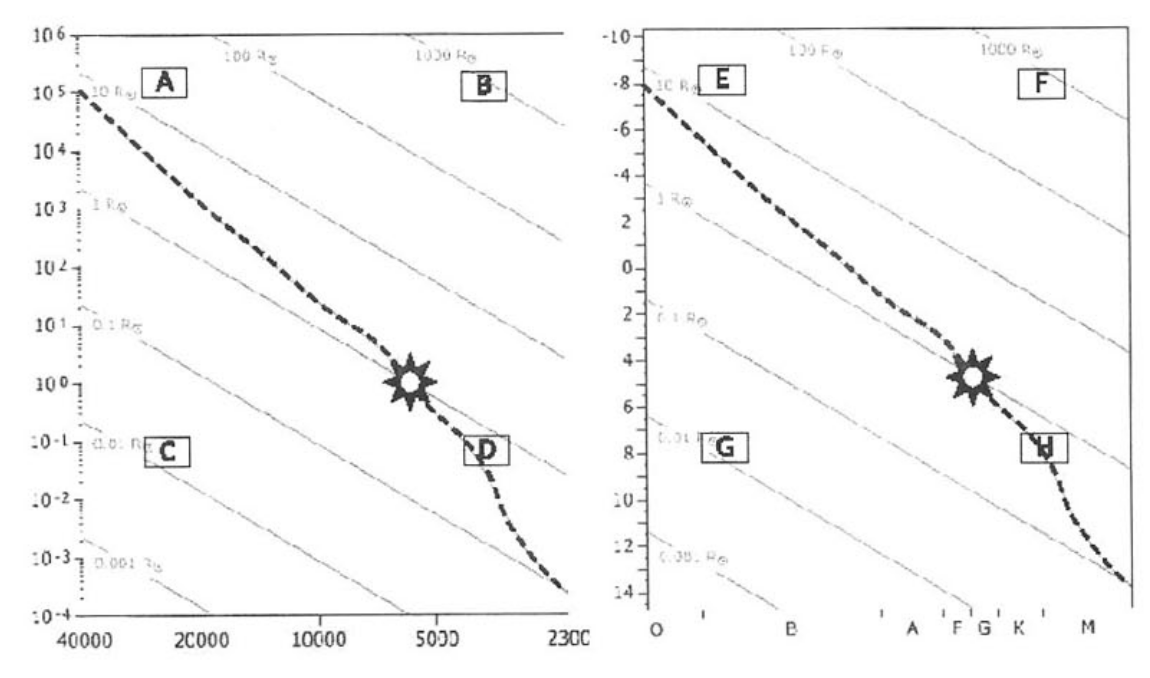
\includegraphics[width=0.9\textwidth]{diagramHR.png}
	%\caption{Foto asli rasi Crux. Oleh Eckhard Slawik.}
	\label{fig:diagramHR}
\end{figure}
Garis tebal putus-putus pada diagram H-R di atas.
\begin{choices}
\item Menyatakan jejak evolusi Matahari dari kiri-atas ke kanan-bawah
\item Menyatakan jejak evolusi Matahari dari kanan-bawah  ke kiri-atas
\item Menyatakan tempat kedudukan bintang-bintang Deret Utama
\item Menandai batas antara bintang-bintang generasi pertama dan kedua
\item Menandai batas antara bintang-bintang dengan dan tanpa medan magnet
\end{choices}


\textit{Jawaban: }C

Rentang temperatur / kelas spektrum yang dilalui garis putus-putus, demikian juga dengan luminositas dan garis-garis radius di dalam diagram HR, mengindikasikan bahwa garis tebal putus-putus tersebut merupakan lokasi bintang-bintang Deret Utama. 


\vspace{1cm}
\textbf{Untuk soal 6 dan 7, jawablah
\begin{choices}
\choice jika 1, 2, dan 3 benar
\choice jika 1 dan 3 benar
\choice jika 2 dan 4 benar
\choice jika 4 saja benar
\choice jika semua benar
\end{choices}}


\question Periode dua \textit{vernal equinox} (titik musim semi) berurutan pada setiap tahun
\begin{enumerate}
\item konstan
\item tidak benar-benar konstan karena terpengaruh oleh nutasi
\item konstan dengan periode selama 1 tahun tropik (yaitu 365,2422 hari)
\item dipengaruhi oleh gangguan gravitasi objek-objek di Tata Surya
\end{enumerate}


\textit{Jawaban: }C

Presisi dan nutasi mengubah orientasi sumbu rotasi Bumi termasuk sudut kemiringan Bumi terhadap ekliptika. Hal ini diakibatkan gangguan gravitasi Matahari dan Bulan bekerja terhadap Bumi yang pepat. Gerak reratanya disebut presesi, sedangkan gerak halusnya disebut nutasi. Nutasi terjadi karena gangguan gravitasinya tidak tetap selama Bumi bergerak mengelilingi Matahari dan Bulan mengelilingi Bumi. Panjang tahun tropis sebenarnya tidak tetap akibat Nutasi dan juga gerak Bumi mengelilingi Matahari yang tidak tetap (akibat gangguan objek-objek Tata Surya).


\vspace{0.5cm}
\question Beberapa hal yang diketahui tentang empat musim di belahan Utara dan Selatan Bumi adalah
\begin{enumerate}
\item perbedaan panjang untuk keempat musim dapat dijelaskan dengan Hukum Kepler
\item dalam waktu belasan ribu tahun, panjang musim dingin dapat menjadi lebih lama dibandingkan dengan panjang musim panas
\item di belahan Utara, panjang musim dingin lebih singkat dibandingkan dengan panjang musim panas
\item faktor paling besar terjadinya empat musim adalah variasi jarak Bumi-Matahari
\end{enumerate}


\textit{Jawaban: }B


Karena orbit Bumi berbentuk elips dan Bumi bergerak lebih cepat di dekat perihelion (Desember-Januari) dibanding aphelion (Juni-Juli), maka durasi musim di belahan Bumi Utara dan Selatan menjadi berbeda. Saat ini misalnya Matahari berada di belahan Bumi utara 7,5 hari lebih lama dibanding di belahan langit Selatan. (Pernyataan 1 dan 3 benar)

Presesi menggeser musim di Bumi, periode presesi sekitar 25800 tahun, sehingga dalam waktu $\sim$13000 tahun, kasus di atas akan terbalik. Pernyataan 2 menyatakan musim dingin lebih lama dibandingkan musim panas tanpa mengaitkan dengan belahan Bumi yang mana, artinya berlaku untuk seluruh Bumi. (Pernyataan 2 salah)


\vspace{1cm}
\textbf{Soal nomor 8, 9, dan 10 dijawab dengan huruf B dan S. Pilihlah B jika pernyataan di soal BENAR. Pilihlah S jika pernyataan di soal adalah SALAH.}


\question Pada diagram HR di soal nomor 5, Betelgeuse adalah bintang maharaksasa yang memiliki radius 1000 kali radius katai putih.


\textit{Jawaban: }S

Seharusnya sekitar 1000 kali radius Matahari (887 \Rsun), bukan 1000 kali radius katai putih.


\vspace{0.5cm}
\question Seorang pendaki naik ke puncak \textit{Mount Everest} yang memiliki ketinggian kurang lebih 8800 m di atas permukaan laut dan memandang ke horizon di permukaan Bumi. Kemudian pendaki tersebut mengukur jarak dari dirinya ke horizon. Di planet Mars, seorang astronot juga mengukur jaraknya ke horizon dari puncak \textit{Mons Elysium} yang memiliki ketinggian 13,8 km di atas rata-rata permukaan Mars. Jarak horizon yang diukur di Mars lebih besar daripada jarak horizon di Bumi.


\textit{Jawaban: }S

Sudut turunnya horizon yang disebabkan ketinggian pengamat dapat dihitung dengan persamaan
$$\cos{\theta} = \frac{R}{R + h}$$
Jarak lurus dari pengamat ke horizon kemudian dapat dicari dengan
$$s = (R+h) \cdot \sin{\theta}$$
atau cara yang lebih mudah, dengan menggunakan hukum Pythagoras langsung
$$s = \sqrt{(R+h)^2 - R^2} = \sqrt{2Rh + h^2}$$

Setelah memasukkan radius planet dan ketinggian pengamat, akan kita peroleh
$s_\oplus = 335,16$ km dan $s_\text{mars} = 306,17$ km. 


\vspace{0.5cm}
\question Fraksi massa gabungan bintang dan gas terhadap massa total galaksi Bimasakti pada jarak 8 kpc dari pusat adalah 52,9\%. Sedangkan sisa massa adalah massa materi gelap (\textit{dark matter}). Distribusi massa materi gelap bersifat simetri bola. Kecepatan rotasi objek pada jarak 8 kpc adalah 220 km/s. Dengan menggunakan tetapan gravitasi $G = 4,302 \times 10^{-3}$ pc $\left( \frac{\text{km}}{\text{s}} \right)^2 M_{\odot}^{-1}$, maka kerapatan materi gelap adalah
$$\rho_{\text{dm}} = 0,02 \text{ } M_{\odot}/\text{pc}^{3}$$


\textit{Jawaban: }B

Massa galaksi hingga radius $R = 8$ kpc dapat dihitung dengan menggunakan kecepatan orbit lingkaran:
\begin{equation*}
M = \frac{v^2 \cdot R}{G} = \frac{220^2 \cdot 8000}{4,302 \times 10^{-3}} = 9 \times 10^{10} M_{\odot} 
\end{equation*}
Kerapatan \textit{dark matter} kemudian dapat dicari,
\begin{equation*}
\rho_{\text{dm}} = \frac{M_{\text{dm}}}{V} = \frac{(1 - 0,529) M}{\frac{4}{3} \pi R^3} = 0,02 \text{ } M_{\odot}/\text{pc}^{3} 
\end{equation*}


\vspace{1cm}
\textbf{Esai Pendek}

\question Sebuah awan berbentuk bola dengan radius $R = 10$ pc memiliki kerapatan molekul hidrogen yang seragam, yaitu $n(H_2)$ = 300 cm$^{-3}$. Berapakah kuat medan magnet $B$ yang diperlukan agar energi magnetik dari awan sama besar dengan energi potensial gravitasinya?

\textit{Petunjuk}: Rapat energi magnetik adalah
$$u_{B} = \frac{B^2}{8\pi}$$


\textit{Jawaban: }

Rapat massa awan berisi molekul Hidrogen ($H_2$):
\begin{eqnarray*}
\rho = \frac{300 \text{  H}_2}{\text{cm}^{3}} = \frac{300 \cdot 2 \cdot 1,6735 \times 10^{-24}}{\text{cm}^{3}} =  \frac{300 \cdot 3,347 \times 10^{-24} \text{  gr}}{\text{cm}^{3}} = 1,0041\times 10^{-21} \frac{\text{gr}}{\text{cm}^3}
\end{eqnarray*}

Energi potensial gravitasi bola gas dengan asumsi kerapatan konstan:
\begin{eqnarray*}
E &=& \frac{3}{5}\frac{GM^2}{R} = \frac{3}{5} \frac{G (\rho V)^2}{R}
\end{eqnarray*}
Rapat energi potensial gravitasi,
\begin{equation*}
u_G = \frac{E}{V} = \frac{3}{5} \frac{G\rho^2 V}{R} = \frac{4}{5} G\rho^2 \pi R^2
\end{equation*}
Hati-hati, rumus rapat energi magnetik yang diberikan di soal merupakan rumus dalam satuan CGS (satuan $u_B$ menjadi erg/cm$^3$), bukan MKS (satuan SI).
\begin{eqnarray*}
u_B &=& u_G \\
\frac{B^2}{8 \pi} &=& \frac{4}{5} G \rho^2 \pi R^2\\
B^2 &=& \frac{32}{5} G \rho^2 \pi^2 R^2\\
B &=& \sqrt{\frac{32 G}{5}} \pi \rho R = \sqrt{\frac{32 \cdot 6,674 \times 10^{-8}}{5}} \cdot \pi \cdot 1 \times 10^{-21} \cdot 3,086 \times 10^{19} \\
B &=& 6,36 \times 10^{-5} \text{   gauss} \qquad = 6,36 \times 10^{-9} \text{  Tesla}
\end{eqnarray*}

\textit{Catatan}: \\
Dalam satuan SI, persamaan rapat energi magnetik (dalam vakum $\rightarrow$ tidak ada materi di dalamnya) adalah:
\begin{equation*}
u_B = \frac{1}{2}\frac{B^2}{\mu_0} = \frac{1}{2}\frac{B^2}{4 \pi \times 10^{-7}} \qquad (\text{Joule m}^{-3})
\end{equation*}
dengan $\mu_0$ adalah \textit{permeability of vacuum}.

Jika dihitung dengan memasukkan $G = 6,674 \times 10^{-11} \frac{  \text{m}^3}{\text{kg s}^2}$, $\rho = 1 \times 10^{-18}$ kg/m$^{3}$, $R = 3,086 \times 10^{17} $ meter, maka akan kita peroleh:
$$B = \sqrt{\frac{32 G \times 10^{-7}}{5}} \pi \rho R  = 6,36 \times 10^{-9} \text{  Tesla}$$ 

\vspace{0.5cm}
\question Pada suatu malam, kamu mengamati Saturnus dengan menggunakan teleskop ($D = 279,4$ mm, $f/D = 10,0$) dan sebuah \textit{eyepiece} dengan medan pandang semu (\textit{apparent Field-of-View}) sebesar 55\de. Data dari almanak astronomi menunjukkan bahwa untuk waktu pengamatan tersebut jarak Bumi dan Saturnus adalah 10,627 sa dan diameter Saturnus beserta cincin yang tampak adalah 278205,221 km.

Hasil pengamatan ditampilkan pada gambar berikut:
\begin{figure}[H]
	\centering
	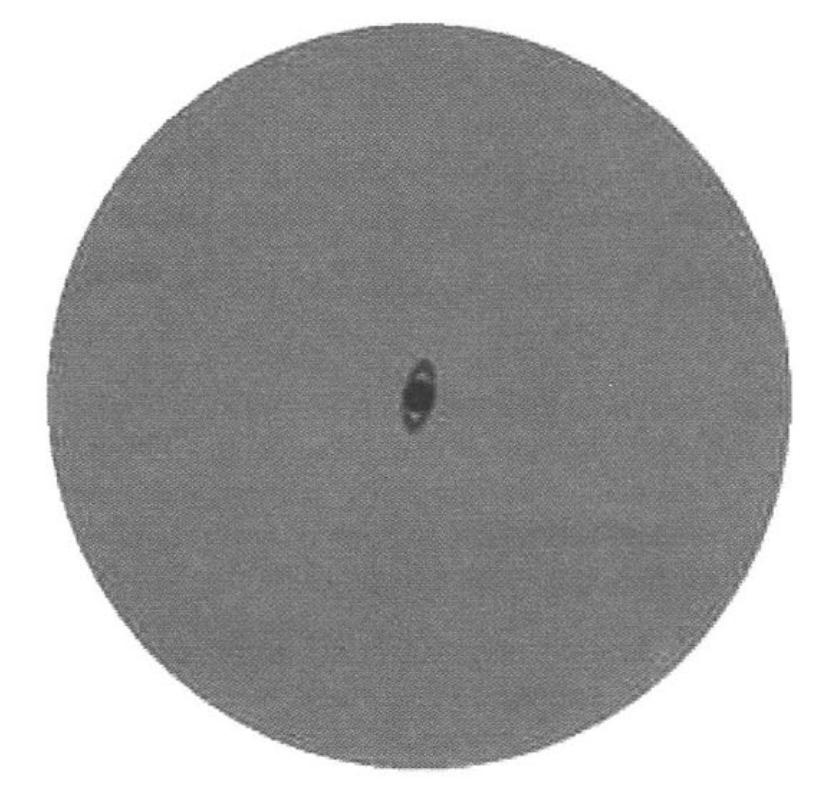
\includegraphics[width=0.5\textwidth]{saturn.png}
	%\caption{Foto asli rasi Crux. Oleh Eckhard Slawik.}
	\label{fig:saturn}
\end{figure}
Dengan bantuan tabel konstanta yang disediakan, tentukanlah:
\begin{enumerate}[a.]
	\item Diameter sudut Saturnus
	\item Medan pandang pada gambar
	\item Panjang fokus \textit{eyepiece} yang digunakan
\end{enumerate}


\textit{Jawaban: }

\begin{enumerate}[a.]
	\item Diameter sudut Saturnus:
	\begin{eqnarray*}
	\theta_\text{saturn} &=& \frac{D}{d}\\
	&=& 0,000174996427744843 \text{  rad} =  0,01^{\circ} = 0,6\am = 36\as
	\end{eqnarray*}
	\item Menggunakan penggaris dan gambar di kertas soal, kita dapat mengukur diameter Saturnus (beserta cincinnya, arah diagonal) untuk kemudian membandingkannya dengan diameter lingkaran \textit{field of view} (fov).
	
	Karena saya tidak punya kertas soal dan penggaris, hanya softcopy hasil scan soal, saya pakai software (\texttt{ImageJ}) untuk mengukur panjang keduanya dalam satuan pixel.
	\begin{eqnarray*}
	\frac{\theta_{\text{fov}}}{\theta_{\text{saturn}}} &=& \frac{D_{\text{fov}}}{D_{\text{saturn}}}\\
	\theta_{\text{fov}} &=&  \frac{D_{\text{fov}}}{D_{\text{saturn}}} \cdot \theta_{\text{saturn}}  = \frac{744 \text{ px}}{75 \text{ px}} \cdot 0,01^\circ = 0,09946^\circ
	\end{eqnarray*}
	\item Panjang fokus \textit{eyepiece} dapat dicari dengan:
	\begin{eqnarray*}
	\theta_\text{fov} &=& \frac{55^\circ}{M} = \frac{55^\circ F_{ok}}{F_{ob}}\\
	F_{ok} &=& \frac{\theta_\text{fov}}{55^\circ} \cdot F_{ob} =  \frac{0,09946}{55^\circ} \cdot 2794 \simeq 5 \text{  mm}
	\end{eqnarray*}
\end{enumerate}


\vspace{0.5cm}
\question Suatu tahun dalam sistem kalender surya dikatakan kabisat bila habis dibagi 4, namun untuk tahun abad (tahun dengan kelipatan 100) dikatakan kabisat hanya jika habis dibagi 400, dan tahun kelipatan 4000 bukan tahun kabisat. Di sistem kalender surya yang lain, suatu tahun juga dikatakan kabisat bila habis dibagi 4, namun untuk tahun abad dikatakan kabisat hanya jika bersisa bagi 200 atau 600 dari hasil pembagian tahun dengan angka 900. Diketahui bahwa untuk kedua kalender surya ini, tahun kabisat dibagi dalam 12 bulan (total hari = 366 hari), sedangkan tahun  basit dibagi dalam 12 bulan (total hari = 365 hari). Andaikan tanggal 1 bulan 1 tahun 2000 kedua sistem kalender jatuh pada hari yang sama, hitunglah
\begin{enumerate}[a.]
	\item setelah tahun 2000, di tahun abad terdekat berapakah kedua sistem penanggalam bersamaan kembali sebagai tahun kabisat?
	\item mulai tahun abad berapakah kedua sistem penanggalan berbeda untuk pertama kali dalam penentuan tahun kabisat?
\end{enumerate}
Sebagai informasi, sistem penanggalan pertama adalah kalender Gregorian (dengan reformasi minor), sedangkan sistem penanggalan kedua adalah kalender gereja Ortodoks Timur (Aveni, A, 1989, \textit{Empires of Time: Calendars, Clocks, and Cultures}, Basic Books Inc. Publ., New York, halaman 118)


\textit{Jawaban: }

Tahun 2000 kedua kalender sepakat bahwa tahun itu merupakan tahun kabisat. 

\begin{enumerate}[a.]
	\item Dicoba satu persatu, diperoleh tahun abad 2400 sebagai tahun kabisat terdekat setelah tahun 2000 untuk kedua kalender.
	\item Dicoba satu persatu, diperoleh tahun abad 2800 sebagai tahun kabisat di kalender gregorian dan tahun basit di kalender Ortodoks Timur; pertama kali berbeda sejak tahun 2000.
\end{enumerate}



\vspace{0.5cm}
\question Jika pada pengamatan fotometri galaksi diperoleh nisbah sinyal terhadap derau ($S/N$) = 5, hitunglah galat magnitudo galaksi tersebut.


\textit{Jawaban: }

Bagi yang masih belum kenal dengan diksi yang digunakan ;)
\begin{itemize}
	\item nisbah = rasio / perbandingan
	\item derau = noise
	\item $S/N$ = \textit{signal to noise ratio}, rasio antara sinyal data dengan \textit{backgound noise}
	\item galat = error / kesalahan pengukuran
\end{itemize}

Diketahui: $ \frac{N}{S} = \frac{\sigma_f}{f} = \frac{1}{5}$

Galat magnitudo dapat dicari dengan,
\begin{eqnarray*}
\sigma_m = m_{f \pm \sigma_f} - m_f = -2,5 \log{\left(\frac{f \pm \sigma_f}{f}\right)} = -2,5 \log{\left(1 \pm \frac{\sigma_f}{f}\right)}
\end{eqnarray*}
sehingga kita peroleh,
\begin{eqnarray*}
	-2,5 \log{\frac{6}{5}} = -0,19795 \qquad \text{atau} \qquad -2,5 \log{\frac{4}{5}} = 0,242275
\end{eqnarray*}
yang kemudian dapat kita rata-ratakan nilai mutlaknya (jika butuh 1 nilai) menjadi galat magnitudo sebesar $\sigma_m$ = 0,22.

\textit{Catatan}:\\
Rumus perambatan kesalahan dari fluks ke magnitudo (hanya berlaku jika $\sigma_f \ll f$):
\begin{equation*}
\vert \sigma_m \vert = 1,086 \frac{\sigma_f}{f}
\end{equation*}


\vspace{0.5cm}
\question Seorang observer mengukur kecerlangan langit dengan Teleskop Zeiss berdiameter 60 cm dan detektor. Diketahui magnitudo kecerlangan langit pada panjang gelombang visual ($\lambda = 5500$ \AA) adalah $m_{\text{sky,V}} = 20,5$ magnitudo per detik busur kuadrat dan \textit{seeing} langit adalah 2\as. Hitunglah jumlah foton tiap detik yang diterima teleskop dari langit dengan \textit{seeing} langit tersebut dan efisiensi teleskop 95\%. Sebagai perbandingan, Matahari memiliki fluks $F_{\odot}=1,6 \times 10^5$ erg cm$^{-2}$ s$^{-1}$. Dalam hal ini, ekstingsi dapat diabaikan dan pengamatan ke arah meredian.


\textit{Jawaban: }

Untuk menghitung jumlah foton yang diterima teleskop tiap detik, kita perlu mengetahui fluks (energi per satuan waktu per satuan luas) yang diterima teleskop dan luas penampangnya.

Luas bukaan teleskop:
\begin{eqnarray*}
	A = \frac{1}{4} \pi D^2 = \frac{1}{4} \pi 60^2 = 2827,43 \text{  cm}^2 
\end{eqnarray*}

Kita asumsikan :) yang dimaksud soal adalah kecerlangan langit sebagai \textit{background source} untuk melakukan koreksi ketika melihat objek titik (\textit{point source}) seperti bintang yang `melebar' sebesar 2\as{} karena \textit{seeing}.
\begin{eqnarray*}
	S &=& m + 2,5\log{(A)}\\
	m &=& S - 2,5 \log{(A)}\\
	m &=& 20,5 - 2,5 \log{(\pi \cdot 1^2)}\\
	m &=& 19,26
\end{eqnarray*}
Fluks langit seluas ini menjadi
\begin{eqnarray*}
m - m_{\odot} &=& -2,5 \log{\frac{F}{F_{\odot}}}\\
17,26 + 26,78 &=& -2,5 \log{\frac{F}{1,6 \times 10^5}}\\
F &=& 6,139 \times 10^{-14} \text{   erg cm}^{-2}\text{ s}^{-1}
\end{eqnarray*}
Jumlah foton:
\begin{eqnarray*}
	N &=& \frac{0,95 \cdot E_\text{terima}}{\frac{hc}{\lambda}} =  \frac{0,95 \cdot F \cdot A \cdot \lambda}{hc}\\
	N &=& 45,658 \quad \text{foton/s} \quad \approx 46 \quad \text{foton/s}
\end{eqnarray*}


\vspace{1.5cm}
\textbf{Esai Panjang}

\question Sebuah elektron pada atom bergerak mengelilingi inti pada lintasan tertentu pada keadaan dasar sehingga elektron memiliki momentum sudut ($L$) sebagai berikut

$$L = m_e v r = \frac{nh}{2\pi}$$

Dalam rumus tersebut, $m_e$ adalah massa elektron, $v$ adalah kecepatan orbit elektron, $r$ adalah radius orbit lingkaran, dan $n$ adalah bilangan bulat berkaitan dengan tingkat energi, dengan $n = 1$ untuk elektron pada keadaan dasar.
\begin{enumerate}[a.]
	\item Jika elektron bergerak dengan orbit lingkaran pada keadaan dasar, tentukan radius orbit elektron dalam satuan meter.
	\item Energi elektron yang mengorbit inti tidak lain adalah energi potensial listrik. Tunjukkan bahwa energi elektron pada suatu tingkat energi berkaitan dengan $n^2$
	\item Jika elektron berpindah dari keadaan dasar ke tingkat energi yang lebih tinggi ($n=2$), tentukan panjang gelombang energi yang diserap elektron untuk berpindah. Berikan jawaban dalam satuan meter.
\end{enumerate}
Sebagai informasi, akibat penyerapan energi, pada pengamatan spektroskopi, akan tampak garis serapan dengan panjang gelombang energi tersebut.


\textit{Jawaban: }

\begin{enumerate}[a.]
	\item Kecepatan orbit elektron
	\begin{eqnarray*}
	F_\text{sentripetal} &=& F_\text{coulomb}\\
	m_e \frac{v^2}{r} &=& \frac{k_e e^2}{r^2}\\
	v &=& e \left( \frac{k_e}{m_e r}\right)^{1/2}
	\end{eqnarray*}
	Dari momentum sudut elektron
	\begin{eqnarray*}
	m_e v r &=& \frac{nh}{2\pi}\\
	m_e e \left( \frac{k_e}{m_e r}\right)^{1/2} r &=& \frac{nh}{2\pi}\\
	m_e e^2 k_e r &=& \frac{n^2h^2}{4\pi^2}\\
	r &=& \frac{n^2h^2}{4\pi^2 m_e e^2 k_e}\\
	r &=& 5,291772 \times 10^{-11} n^2 \quad \text{meter} \quad = 0,529 n^2 \quad \text{\AA}
	\end{eqnarray*}
	Untuk $n=1$ maka $r = 5,291772 \times 10^{-11}$ meter
	\item Energi elektron
	\begin{eqnarray*}
	E &=& E_k + E_p = \frac{1}{2} m_e v^2 - \frac{k_e e^2}{r} = \frac{1}{2} m_e \frac{k_e e^2}{m_e r} - \frac{k_e e^2}{r} = \frac{1}{2} \frac{k_e e^2}{r} - \frac{k_e e^2}{r}\\
	E &=& -\frac{k_e e^2}{2r}\\
	E &=& -\frac{2\pi^2 e^4 m_e k_e^2}{n^2 h^2}\\
	E &=& - \frac{2,179872 \times 10^{-18}}{n^2} \quad \text{Joule} \quad = - \frac{13,6}{n^2} \quad \text{eV} 
	\end{eqnarray*}
	Terbukti bahwa tingkat energi elektron berkaitan dengan $n^2$.
	\item Untuk pindah dari tingkat energi $n$ ke tingkat energi $m$, maka energi yang dibutuhkan (diserap) atau dikeluarkan besarnya adalah
	\begin{eqnarray*}
		\Delta E &=& E_m - E_n\\
		\frac{hc}{\lambda} &=& 2,179872 \times 10^{-18} \left( \frac{1}{n^2} - \frac{1}{m^2} \right) \\
		\frac{1}{\lambda} &=& 10973732 \left( \frac{1}{n^2} - \frac{1}{m^2} \right) \text{  meter}^{-1} \quad \text{atau} \quad \lambda = \frac{911,27}{\left( \frac{1}{n^2} - \frac{1}{m^2} \right)} \text{  \AA} \quad \text{(hafalan penulis :v)}
	\end{eqnarray*}
	Panjang gelombang energi yang diserap untuk elektron pindah dari kulit $n=1$ ke $n=2$ adalah $1,215 \times 10^{-7}$ meter.
\end{enumerate}


\vspace{0.5cm}
\question Jika di antara bintang dan pengamat terdapat materi antar bintang yang menyebabkan intensitas suatu cahaya berkurang sebesar 1\% setiap 100 pc.
\begin{enumerate}[a.]
\item Tentukan berapa jarak yang ditempuh cahaya dalam menembus materi antar bintang sehingga intensitasnya menjadi setengah dari intensitas semula saat dipancarkan. Asumsikan tidak ada proses hamburan di antara bintang dan pengamat, hanya absorpsi. Berikan jawaban dalam satuan meter.
\item Dengan mengandaikan intensitas bintang mengalami peredaman secara eksponensial dengan faktor $\tau$ (dalam astronomi $\tau$ dikenal sebagai tebal optis), hitunglah nilai $\tau$ jika cahaya menempuh jarak 1 kpc.
\end{enumerate}


\textit{Jawaban: }

\begin{enumerate}[a.]
	\item Setiap 100 pc intensitas cahaya berkurang menjadi 0,99 kali sebelumnya. Jika kita tuliskan persamaannya,
	\begin{eqnarray*}
		I &=& 0,99^{\frac{d}{100}} I_0 \\
		0,5 &=& 0,99^{\frac{d}{100}}\\
		d &=& 100 \cdot \frac{\log{0,5}}{\log{0,99}}\\
		d &=& 6896,756 \text{  pc}
	\end{eqnarray*}

	
	\item Intensitas cahaya berkurang secara eksponensial, bergantung pada sifat materi penyerap ($k \rightarrow$ rapat jumlah dan ukuran partikel) serta jarak tempuh cahaya (atau tebal materi penyerap) $d$.
	\begin{eqnarray*}
		I_\text{out} &=& I_\text{in} e^{-\tau}\\
		I_\text{out} &=& I_\text{in} e^{- k d}\\
		0,99 I_\text{in} &=& I_\text{in} e^{- k \cdot 100}\\
		k &=& - \frac{\ln{(0,99)}}{100} = 0,0001005033585350145
	\end{eqnarray*}
	
	Tebal optis untuk jarak 1 kpc,
	\begin{eqnarray*}
		\tau &=& kd = 0,0001005033585350145 \cdot 1000 \simeq 0,1
	\end{eqnarray*}
\end{enumerate}


\vspace{0.5cm}
\question Salah satu kelompok galaksi yang paling terkenal adalah ``Stephan's Quintet'' (lihat gambar) ditemukan oleh astronom Perancis \'{E}douard Stephan pada tahun 1877. Terdapat 5 buah galaksi spiral dan eliptikal yang tergabung dalam kelompok tersebut. Kemudian ternyata ditemukan ada galaksi lain di dekatnya, NGC 7320C, yang lebih kecil dan mungkin juga terkait dengan kelompok galaksi ini. Di dalam tabel, diberikan data nama galaksi, tipe morfologi menurut Vaucouleurs, koordinat ekuator dan kecepatan radial dalam \kms.

\begin{table}[H]
\centering
\small
\begin{tabular}{|l|c|c|c|c|}
	\hline
	Nama galaksi & Tipe morfologi & \alp{} (J2000.0) & \del{} (J2000.0) & Kecepatan radial\\ 
	& & & & (\kms) \\
	\hline
	\hline
	NGC 7317 & E4 & 22\jam35\m51,9\s & +33\de56\am42\as & 6599 \\
	\hline
	NGC 7318A & E2pec & 22\jam35\m56,7\s & +33\de57\am56\as & 6630 \\
	\hline
	NGC 7318B & SB(s)bc pec & 22\jam35\m58,4\s & +33\de57\am57\as & 5774 \\
	\hline
	NGC 7319 & SB(s)bc pec & 22\jam36\m3,5\s & +33\de58\am33\as & 6747 \\
	\hline
	NGC 7320 & SA(s)d & 22\jam36\m3,4\s & +33\de56\am53\as & 786 \\
	\hline
	NGC 7320C & (R)SAB(s)0/a & 22\jam36\m20,4\s & +33\de59\am6\as & 5985 \\
	\hline
\end{tabular}
\end{table}

\begin{figure}[H]
	\centering
	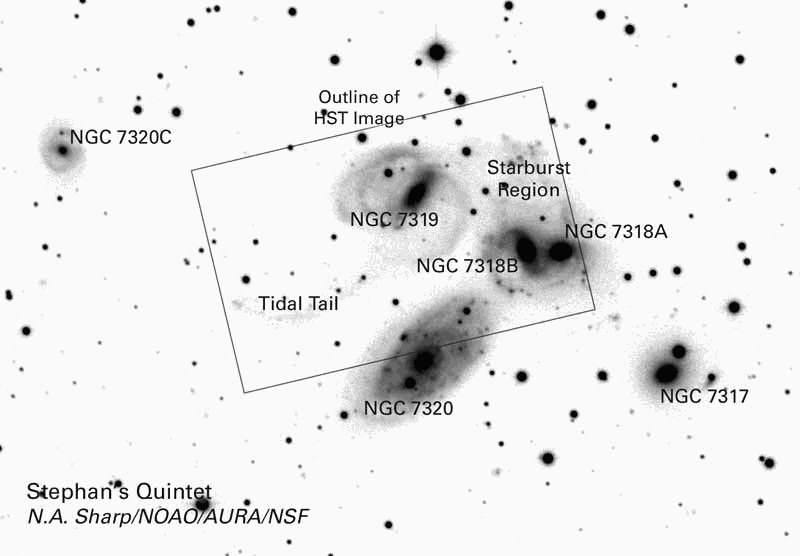
\includegraphics[width=0.85\textwidth]{gugus_galaksi.png}
	%\caption{Foto asli rasi Crux. Oleh Eckhard Slawik.}
	\label{fig:diagramHR}
\end{figure}

\begin{enumerate}[a.]
	\item Tentukan apakah ada salah satu galaksi sebenarnya tidak terikat secara gravitasi ke kelompok tersebut?
	\item Manakah dari kedua galaksi ini memiliki ukuran sejati lebih besar, NGC 7320 atau NGC 7320C?
	\item Dengan menggunakan teorema virial yang menyatakan bahwa energi kinetiknya adalah setengah dari energi potensial gravitasi, hitunglah massa kelompok galaksi tersebut.
\end{enumerate}
\textit{Petunjuk}: Energi total per satuan massa adalah
$$E_{\text{total}} = E_{\text{kinetik}} + E_{\text{potensial}} = \frac{1}{2} \left< v^2 \right> - \frac{3}{5}\frac{GM}{\left< R \right>}$$

dengan $\left< v^2 \right>$  adalah dispersi atau variansi kecepatan, $M$ adalah massa sistem, dan $\left< R \right>$ adalah jarak rata-rata dari pusat sistem.


\textit{Jawaban: }

\begin{enumerate}[a.]
	\item Dari data kecepatan radial (redshift/jarak radial) yang jauh lebih kecil (786 km/s) dibanding galaksi-galaksi lain dapat diketahui bahwa galaksi \underline{NGC 7320} tidak terikat secara gravitasi dengan yang lain. 
	
	Galaksi lain memiliki kecepatan radial (redshift/jarak radial) lebih besar dan saling berdekatan, sekitar 6500 km/s. 
	
	\item Dengan asumsi bahwa kecepatan radial yang diberikan adalah seluruhnya akibat pengembangan alam semesta dengan $H_0 = 69,3$ km/s/Mpc, kita dapat memperkirakan jarak galaksi,
	\begin{equation*}
	d = \frac{v_r}{H_0}
	\end{equation*}
	akan kita peroleh, $d_\text{NGC 7320} = 11,342$ Mpc, dan $d_\text{NGC 7320C} = 86,364$ Mpc.
	
	Sama seperti soal sebelumnya, diameter galaksi (sumbu panjang) dapat kita ukur menggunakan penggaris pada kertas soal, akan tetapi saya menggunakan software \texttt{ImageJ} untuk mengukurnya dalam satuan pixel. Saya peroleh diameter sudut galaksi dalam pixel: 196 px dan 64 px.
	
	Skala citra dapat kita ukur dengan membandingkan jarak sudut antara dua galaksi (dari data posisi) dengan jarak yang kita ukur menggunakan penggaris. Dalam hal ini saya peroleh bahwa jarak sudut antara galaksi NGC 7319 dengan NGC 7320C sebesar 212,784\as{} terwakili oleh jarak 355 px di citra, sehingga saya peroleh skala 0,6 \as/pixel. Diameter sudut galaksi dalam detik busur dapat dihitung: 117,6\as{} dan 38,4\as{}.
	
	Diameter sebenarnya galaksi kemudian dapat kita hitung,
	\begin{eqnarray*}
		D = \theta_\text{(rad)} \cdot d
	\end{eqnarray*}
	hasilnya, $D_\text{NGC 7320} = 6,5 \text{ kpc}$, dan $D_\text{NGC 7320 C} = 16,08 \text{  kpc}$. Galaksi NGC 7320C lebih besar dibanding NGC 7320.
	
	\vspace{0.3cm}
	\textit{Catatan}:
	\begin{itemize}[]
		\item Sebetulnya dengan asumsi dasar di atas, kita tidak perlu menghitung ukuran/diameter sejati galaksi untuk mengetahui galaksi mana yang lebih besar. Cukup dengan membandingkan jarak dan ukuran/diameter yang kita ukur dengan penggaris. Ukuran tampak (diameter sudut) NGC 7320 tiga kali lebih besar, tapi jaraknya 7,6 kali lebih dekat, sehingga dapat disimpulkan bahwa ukuran sejati NGC 7320 lebih kecil dibanding NGC 7320C.
		\item Asumsi kosmologi apa saja yang kita gunakan ketika menggunakan dua rumus yang ditulis di atas?
	\end{itemize}

	\vspace{0.3cm}
	\item Untuk menghitung jarak dari pusat cluster yang kita bisa lakukan misalnya: 
	\begin{enumerate}[(1)]
		\item menggunakan jarak tangensial saja dengan asumsi jarak radialnya ke kita sama besarnya (ambil nilai $v_\text{radial}$ rata-rata). Jarak ke pusat gugusnya perlu dikoreksi $r = \sqrt{2r_\text{t}^2}$; dengan asumsi rata-rata jarak radialnya sama dengan jarak tangensial (bola).
		\item kita pakai asumsi kecepatan peculiarnya nol terlebih dahulu, lalu kita hitung jarak radial ke Bumi menggunakan kecepatan radial masing-masing galaksi (menggunakan hukum Hubble). Kemudian ditambah dengan data jarak tangensial (jarak sudut) untuk mencari jarak masing-masing galaksi ke pusat massanya.
	\end{enumerate}

	Baik cara (1) atau (2) kita dapat gunakan asumsi bahwa massa kelima anggota galaksi sama besar. Untuk memudahkan penentuan pusat massa dan perhitungan jaraknya, perlu diubah dulu dari koordinat bola ke koordinat kartesian. Jika menggunakan cara (1) akan kita peroleh jarak rata-rata ke pusat massa galaksi sekitar 2,62 Mpc. Jika menggunakan cara (2), akan diperoleh jarak rata-rata ke pusat massa gugus galaksi sekitar 5,88 Mpc. 
	
	
	Taksiran besaran ini lumayan berbeda karena terlalu banyak asumsi dan jumlah galaksinya sedikit, dan untuk cara (2) kita mengabaikan efek pengembangan alam semesta terhadap perhitungan jarak radial antar mereka sendiri, serta mengabaikan kecepatan peculiar masing-masing galaksi, yang kontradiktif dengan langkah berikutnya, menjadikan dispersi kecepatan radial galaksi sebagai kecepatan `peculiar' untuk dimasukkan dalam persamaan teorema virial.

	
	Berikutnya kita perlu menghitung dispersi kecepatan galaksi relatif terhadap pusat massa.
	\begin{itemize}
		\item Kecepatan radial rata-rata (kecepatan sistem), $v_\text{sys} = \overline{v} = $ 6347 km/s 
		\item Dispersi kecepatan radial, 
		$$ \left< {v_\text{r}}^2 \right> = \frac{\sum_{i=1}^{N} \left( v_\text{r} - \overline{v} \right)^2}{N} = 152593,2 \times 10^{6} \qquad \text{m}^2\text{s}^{-2}$$
		\item Setelah dilakukan pengukuran dan perhitungan di atas, maka dapat kita gunakan rumus yang diberikan di soal terkait teorema virial. Asumsi lain yang digunakan yaitu kecepatan galaksi di dalam gugusnya bersifat isotropik, sehingga dispersi kecepatan sebenarnya (3D) adalah 3 kali dispersi kecepatan radial.
		\begin{eqnarray*}
			2 E_\text{kinetik} &=& - E_\text{potensial}\\
			\left< v^2 \right> &\approx& \frac{3}{5}\frac{GM}{\left< R \right>}\\
			M &\approx& \frac{5}{3} \frac{\left< v^2 \right> \left< R \right>}{G}\\
			M &\approx& \frac{5}{3}  \frac{ 3 \left<{v_{r}}^2 \right> \left< R \right>}{G}\\
			\text{Cara (1)} & & \\
			M &=& 9,24 \times 10^{44} \quad \text{kg} \quad \approx \quad  4,65 \times 10^{14} \Msun\\
			\text{Cara (2)} & & \\
			M &=& 2,07 \times 10^{45} \quad \text{kg} \quad \approx \quad  1 \times 10^{15} \Msun
		\end{eqnarray*}
	\end{itemize}
	
	
	\textit{Catatan:}
	\begin{itemize}
		\item Bagaimanapun cara yang dipilih, asalkan dituliskan alasan dan asumsi-asumsi yang digunakan (dan asumsinya wajar), diperbolehkan untuk menjawab soal esai seperti ini.
		\item Penggunaan teorema virial untuk menghitung massa memang buanyak asumsinya, termasuk dari rumus awal yang diberikan ;) 
	\end{itemize}
	
\end{enumerate}


\vspace{0.5cm}
\question HD 80715 (BF Lyn dalam \textit{Galactic Catalogue of Variable Stars}) yang berada di konstelasi Lynx adalah sistem bintang ganda spektroskopi bergaris ganda yang berjarak 80 tahun cahaya dari kita. Kedua komponen dalam sistem bintang ganda dekat ini mirip, dengan kelas spektral K3 V.

Gambar di bawah ini menunjukkan perubahan dari waktu ke waktu (dinyatakan dalam angka dengan satuan hari, di sebelah kanan garis spektrum) dari suatu garis absorpsi dalam spektrum bintang yang teramati. Terlihat bahwa pada rentang tertentu, garis spektral terbagi menjadi dua komponen $\lambda_1$ dan $\lambda_2$, kemudian mereka disatukan kembali menjadi satu dengan $\lambda_0$ adalah panjang gelombang saat konfigurasi kedua komponen pada fase orbit kuadratur (segaris) dilihat dari pengamat. Asumsikan bidang orbit tegak lurus bidang pandang pengamat.

\begin{figure}[H]
	\centering
	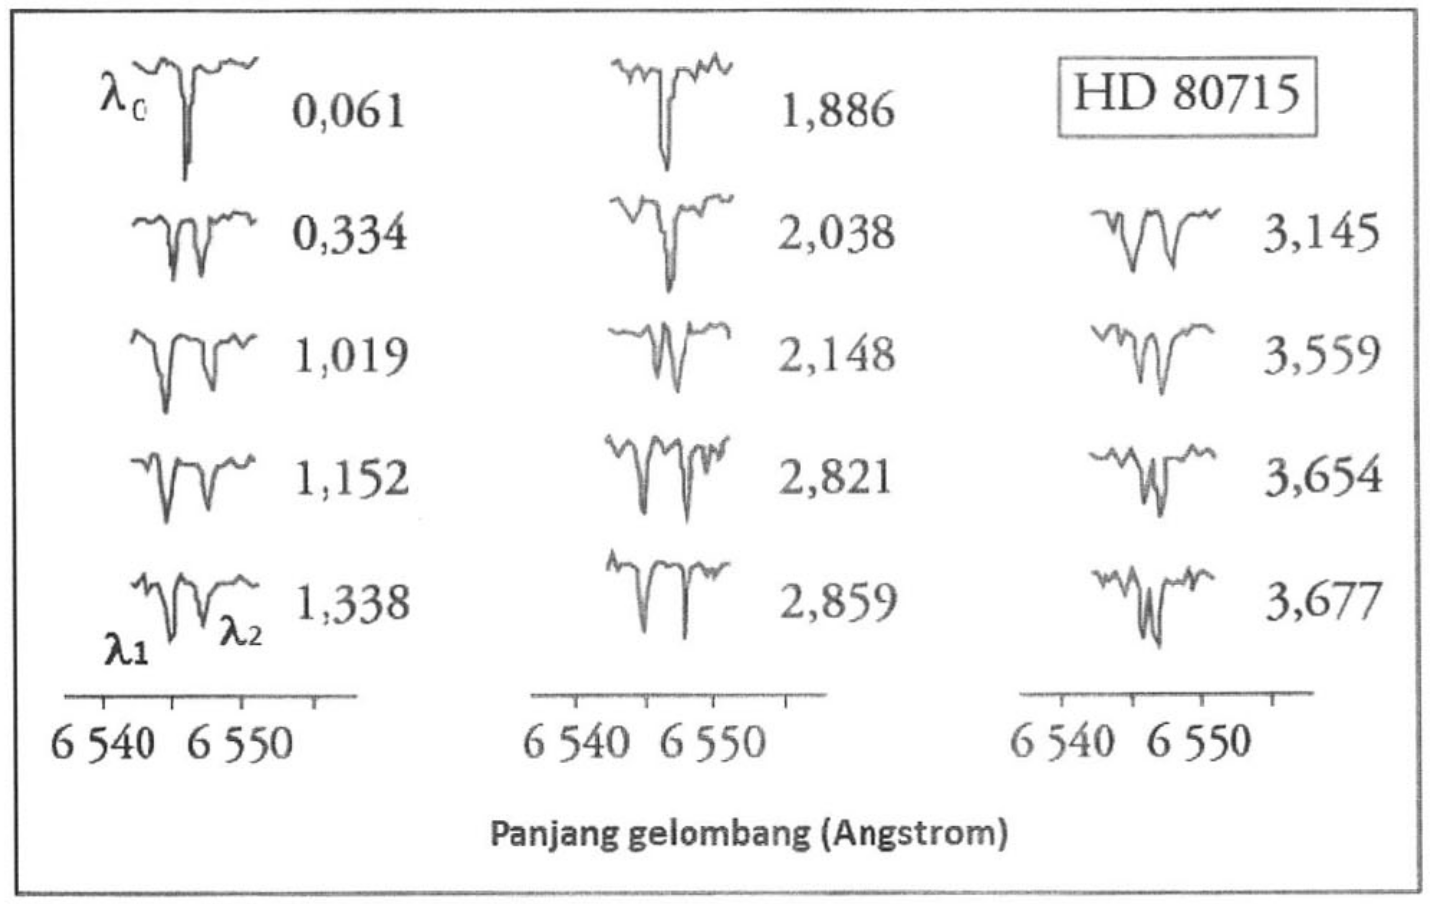
\includegraphics[width=\textwidth]{HD80715.png}
	\label{fig:hd80715}
\end{figure}

\begin{enumerate}[a.]
	\item Ukurlah $\lambda_1$ dan $\lambda_2$ relatif terhadap $\lambda_0$. Perhatikan skala panjang gelombang. Ubahlah hasil pengukuran ini ke kecepatan radial dinyatakan dalam \kms
	\item Bangunlah kurva kecepatan radial, yakni kurva hubungan kecepatan radial terhadap waktu. Pada kurva ini gambarlah kurva sinusoidal yang paling sesuai menurutmu. Nyatakan persamaan sinusoidal untuk masing-masing komponen.
	\item Dari kurva sinusoidal ini, tentukanlah amplitudo kecepatan  radial (satuan \kms) masing-masing komponen dan periode orbit (satuan hari) sistem bintang ganda ini.
	\item Hitung jarak antara dua bintang, nyatakan dalam satuan astronomi (sa).
	\item Temukan massa masing-masing bintang dalam satuan massa Matahari ($M_\odot$).
\end{enumerate}

\textit{Jawaban: }

Seperti pada soal sebelumnya, skala dan jarak antara garis absorpsi dapat diukur dengan menggunakan penggaris pada kertas soal. Untuk keperluan ini saya memanfaatkan aplikasi online yang bisa digunakan untuk mendigitasi gambar plot: \url{https://apps.automeris.io/wpd/}. Untuk membedakan mana bintang 1 dan 2, perhatikan bahwa kedalaman garis absorpsinya berbeda.

Perlu diperhatikan bahwa karena di soal dibilang kedua bintang mirip, \textit{kita bisa asumsikan di awal bahwa kedua bintang massanya sama}. Maka masalah ini dapat menjadi lebih sederhana, cukup dengan mengukur jarak dua garis absorpsi dan membaginya menjadi dua. Hal ini bisa dilakukan jika ternyata ketika mengukur dengan penggaris mengalami kesusahan atau waktu pengerjaannya sudah mepet. ;)

\begin{enumerate}[a).]
	\item Kita tidak diberitahu $\lambda_0$ garis absorpsi yang sebenarnya, walaupun bisa ditebak kemungkinan besar adalah garis H$_{\alpha}$. Oleh karena itu kita gunakan $\lambda_0$ yang ada di gambar saja, di mana panjang gelombang itu mewakili kecepatan sistem terhadap kita. Jika dihitung relatif terhadap $\lambda_0$ tersebut, maka yang kita peroleh adalah kecepatan masing-masing bintang relatif terhadap sistemnya (pusat massa). Walaupun hal tersebut kurang tepat; seharusnya perhitungan dilakukan menggunakan $\lambda_0$ garis absorpsi yang asli, perbedaanya akan kecil. Dari aplikasi online di atas, dapat saya peroleh tabel berikut:
	\begin{table}[H]
		\centering
		\small
		\begin{tabular}{|l|c|c|c|c|}
			\hline
			$t$ & $\Delta \lambda_1$ & $\Delta \lambda_2$ & $v_{r,1}$ & $v_{r,2}$ \\
			\hline
			\hline
			0,061  &  0,140  &  -0,140  &  6,427  &  -6,427  \\
			0,334  &  0,998  &  -0,998  &  45,717  &  -45,712  \\
			1,019  &  1,786  &  -1,523  &  81,796  &  -69,740  \\
			1,152  &  1,402  &  -1,560  &  64,202  &  -71,446  \\
			1,338  &  1,021  &  -1,256  &  46,770  &  -57,513  \\
			1,886  &  0,607  &  0,263  &  27,806  &  12,032  \\
			2,038  &  0,706  &  0,989  &  32,335  &  45,311  \\
			2,148  &  -0,225  &  1,230  &  -10,301  &  56,343  \\
			2,821  &  -1,306  &  1,886  &  -59,809  &  86,385  \\
			2,859  &  -1,207  &  1,779  &  -55,280  &  81,487  \\
			3,145  &  -0,891  &  1,864  &  -40,820  &  85,354  \\
			3,559  &  -0,386  &  1,124  &  -17,691  &  51,484  \\
			3,654  &  -0,091  &  1,005  &  -4,183  &  46,030  \\
			3,677  &  -0,287  &  0,743  &  -13,122  &  34,014  \\
			\hline		
		\end{tabular}
	\end{table}

	\item Kurva kecepatan radialnya dapat diplot kemudian dikira-kira fungsi sinusoidal yang mewakili.
	Gambar di bawah adalah plot kecepatan radial beserta hasil fittingnya, (\textit{atas}) dipisah untuk masing-masing komponen, (\textit{bawah}) kurva rerata jika mengambil asumsi di awal massa bintang sama $m_1 = m_2$ (saya plot salah satu komponen saja). 
	\begin{figure}[!ht]
		\centering
		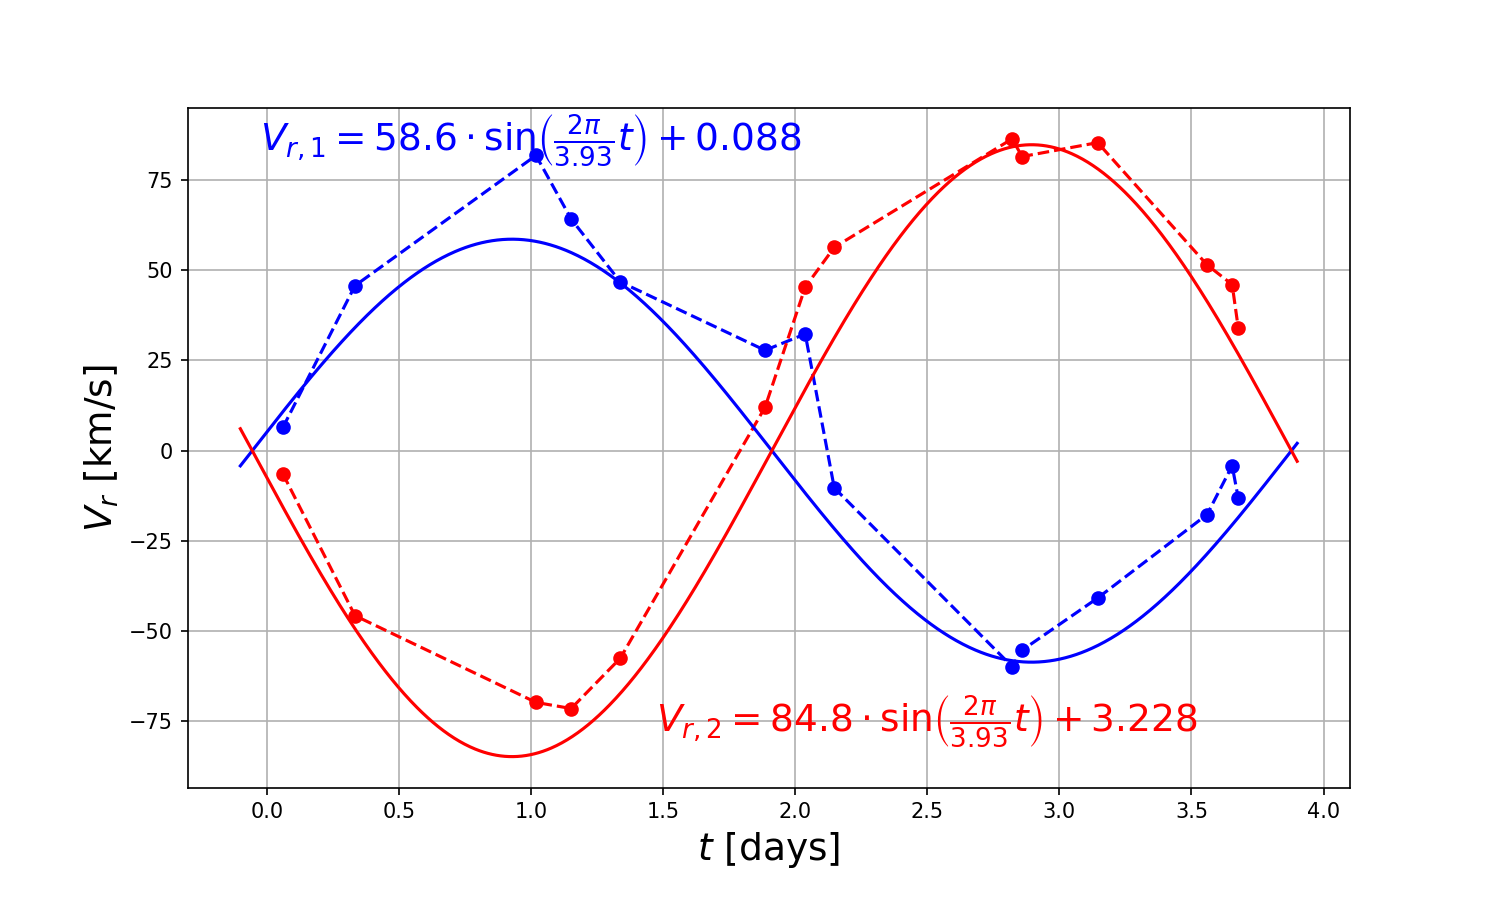
\includegraphics[width=0.65\textwidth]{vrad.png}
		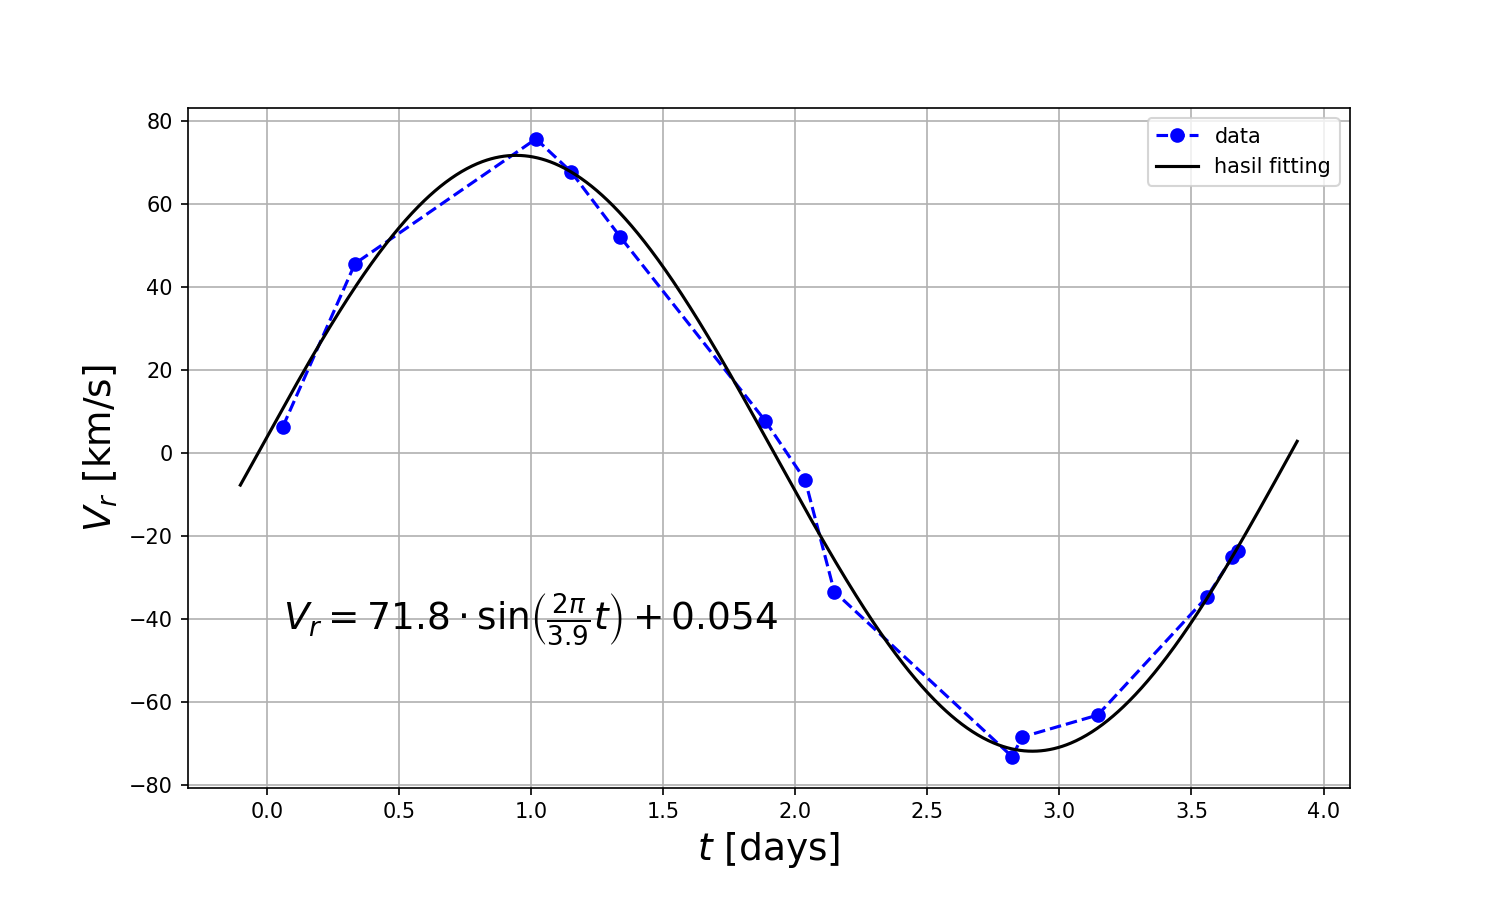
\includegraphics[width=0.65\textwidth]{vrad_combine.png}
	\end{figure}

	\item Kecepatan bintang, $v_1 = 58,6$ km/s, $v_2 = 84,8$ km/s, $P = 3,93$ hari. Jika mengambil asumsi di awal, $v_1 = v_2 = 71,8$ km/s.
	
	\item Jarak antara dua bintang,
		\begin{eqnarray*}
			v_1 = \frac{2 \pi r_1}{P} &\qquad& v_2 = \frac{2 \pi r_2}{P}  \\
			r_1 + r_2 &=& \frac{P}{2 \pi}(v_1 + v_2)\\
			a &=& 7749533,8 \text{   km}  =  0,0518 \text{  sa}
		\end{eqnarray*}
	
	\item Massa masing-masing bintang dapat dicari menggunakan hukum Kepler ($a$ dalam sa, $P$ dalam tahun, $M$ dalam \Msun),
		\begin{eqnarray*}
			\frac{a^3}{P^2} &=& (M_1 + M_2)\\
			M_1 + M_2 &=& 1,2 M_{\odot} \quad \text{dan} \quad \frac{M_1}{M_2} = \frac{v_2}{v_1} = 1,447 \\
			M_1 = 0,7 M_{\odot} &\text{dan}& M_2 = 0,5 M_{\odot}
		\end{eqnarray*}
	Tentu jika kita mengambil asumsi di awal, akan kita peroleh $M_1 = M_2 = 0,6 M_{\odot}$.
		
\end{enumerate}


\vspace{0.5cm}
\question Teori Relativitas Khusus Einstein berlaku untuk berbagai pengamatan, baik di Bumi maupun di angkasa luar. Dua pengamat akan mencatat waktu yang berbeda untuk pengamat yang tinggal di permukaan Bumi terhadap pengamat rekannya yang diam dalam sebuah roket di angkasa luar. Perbedaan waktu yang tercatat oleh kedua pengamat, dinyatakan dalam persamaan berikut:

$$t_1 = t_2 \sqrt{ 1 - \frac{2GM}{Rc^2} }$$

$t_1 = $ waktu diukur oleh pengamat yang berada di permukaan sebuah planet atau bintang (dalam detik)

$t_2 = $ waktu diukur oleh pengamat yang berada di angkasa luar (dalam detik)

$\sqrt{1 - 2GM/(Rc^2)}$ adalah faktor dilatasi waktu bagi pengamat yang berada pada jarak $R$ dari planet atau bintang.

$M$ = massa planet atau bintang dalam kilogram

$R$ = jarak planet atau bintang ke pengamat di angkasa luar

Jika seorang astronot bisa berada di permukaan bintang netron ($M = 2,16 \times 10^{30}$ kg, berjejari $r=10$ km) mencatat durasi satu kejadian dan mengukur waktu tepat 60 menit untuk kejadian yang terlihat olehnya.
\begin{enumerate}[a.]
\item Berapa durasi waktu yang dicatat oleh pengamat kedua yang juga melihat kejadian sama dan berada pada jarak 20 km dari pusat bintang, sebelum keduanya berkomunikasi membandingkan pencatatan durasi kejadian itu?
\item Hitung rasio (perbandingan) faktor dilatasi waktu pada pengamat pertama dan kedua.
\item Dilatasi waktu menyebabkan sinyal cahaya atau sinyal radio yang berasal dari pemancar pengamat di angkasa luar ke alat penerima pengamat yang ada di bintang kompak, tidak lagi merambat sejauh 20 km tetapi lebih besar dari 20 km. Hitung pertambahan jarak itu.
\end{enumerate}


\textit{Jawaban: }

Persamaan \textit{gravitational time dilation} yang diberikan di soal dapat ditulis ulang menjadi:
\begin{equation*}
t = t_0 \sqrt{1 - \frac{r_s}{r}} 
\end{equation*}
dengan $r_s$ (Schwarzchild's radius),
\begin{equation*}
r_s = \frac{2GM}{c^2} = 3207,995489997936 \text{   meter}
\end{equation*}
dan $t_0$ adalah waktu yang diukur pengamat di angkasa luar yang `jauh' dari massa sumber gravitasi ($r \ggg $),
\begin{eqnarray*}
	t_0 &=& \frac{t_1}{\sqrt{1 - \frac{r_s}{r_1}}}\\
	t_0 &=& 4368,2101 \text{   s} = 72,803502 \text{   m}
\end{eqnarray*}

Untuk bahan diskusi:
\begin{itemize}
	\item Apa yang terjadi jika kita mengambil nilai $r < r_s$?
	\item Persamaan di atas mirip sekali dengan persamaan dilatasi waktu pada kasus relativitas khusus, yaitu dengan mengganti $v$ di dalam faktor Lorentz $\gamma = \frac{1}{\sqrt{1 - \frac{v^2}{c^2}}}$ dengan kecepatan lepas di $r$. 
\end{itemize}

\begin{enumerate}[a.]
	\item Waktu yang diukur pengamat kedua, 
	\begin{eqnarray*}
		t_2 &=& t_0 \sqrt{1 - \frac{r_s}{r_2}}\\
		t_2 &=& 4002,5779 \text{   s} = 66,709631 \text{   m}
	\end{eqnarray*}
	
	\item Perbandingan faktor dilatasi waktu pengamat pertama ($r_1 = 10$ km) dan kedua ($r_2 = 20$ km); $r_2 = 2r_1$. 
	\begin{equation*}
	\frac{t_1}{t_2} = \frac{60}{66,709631} = 0,89942035 \simeq 0,9
	\end{equation*} 
	atau dengan cara yang lebih panjang :v
	\begin{eqnarray*}
	\frac{\sqrt{1 - \frac{2GM}{r_1c^2}}}{\sqrt{1 - \frac{2GM}{r_2c^2}}} &=& \sqrt{ \frac{1 - \frac{r_s}{r_1}}{1 - \frac{r_s}{r_2}} } = \sqrt{ \frac{1 - \frac{r_s}{r_1}}{1 - \frac{r_s}{2 r_1}} } = \sqrt{ \frac{\frac{r_1 - r_s}{r_1}}{\frac{2r_1 - r_s}{2 r_1}} } = \sqrt{ \frac{r_1 - r_s}{r_1} \cdot \frac{2 r_1}{2r_1 - r_s} } \\ 
	&=& \sqrt{2} \sqrt{\frac{r_1 - r_s}{2r_1 - r_s}} =  \sqrt{2} \sqrt{\frac{10000 - 3207.995489997936}{20000 - 3207.995489997936}}\\
	&=& 0,89942035 \simeq 0,9
	\end{eqnarray*}
	
	\item Jika melihat soal sebelumnya, soal ini terlihat agak aneh. Alternatif pemahaman soal:
	\begin{enumerate}[1).]
		\item Jarak 20 km yang dimaksud adalah jarak dari pemancar ke pusat bintang netron. \textit{Masalah}: apakah ada pengamat/penerima sinyal di pusat bintang netron? Jika kita paksakan, karena $r < r_s$ solusi yang kita peroleh menjadi imajiner.
		\item Jarak yang dimaksud adalah dari pengamat kedua ke pengamat pertama (dipermukaan). \textit{Masalah}: Untuk kasus ini di soal harusnya tertulis jarak 10 km, bukan 20 km.
		\item Jarak yang dimaksud adalah dari pengamat di $r=30$ km ke $r=10$ km (dipermukaan).
		\item Jarak yang dimaksud adalah jarak dari radius Schwarzschild $r=r_s$ ke $r=20$ km. \textit{Masalah}: tidak disebutkan secara eksplisit; $r_s$ ada di `dalam' bintang netron.
		\item Jarak yang dimaksud adalah jarak ke permukaan bintang netron tapi tidak dalam arah radial, melainkan miring (+melengkung) sehingga tetap 20 km. \textit{Masalah}: mungkinkah konfigurasi ini? Kalaupun mungkin, akan lebih susah mencari solusinya ;)
	\end{enumerate}
	
	%Jika sudah belajar relativitas khusus (ada di kurikulum Fisika SMA), kita mengenal dilatasi waktu dan kontraksi panjang yang persamaannya `terbalik'. Hal ini sebetulnya sama berlakunya untuk kasus ini. 
	
	Kasus ini terkait dengan penggambaran ruang-waktu di sekitar massa berbentuk bola yang diam (tidak berotasi/kencang + tidak ada muatan). Geometri ruang-waktunya dapat digambarkan dengan geometri Schwarzschild, yang dapat dituliskan sebagai berikut (untuk kenalan saja; dalam koordinat bola):
	\begin{equation*}
		ds^2 = -c^2 d\tau^2 = - \left( 1 - \frac{r_s}{r} \right) c^2 dt^2 + \left(1 - \frac{r_s}{r} \right)^{-1} dr^2 + r^2 \left( d\theta^2 + \sin^2\theta d\varphi^2 \right)
	\end{equation*}
	Dapat dilihat dari mana rumus yang diberikan di soal berasal.
	
	``Ruang  Schwarzschild'' ini bersifat isotropik, tetapi tidak homogen. Menurut metrik Schwarzschild di atas, jarak proper (dalam arah radial); jarak sebenarnya jika kita ukur menggunakan penggaris dan kita hentikan waktunya, akan bergantung pada koordinat $r$ di dalam metrik, dengan hubungan $dr / \sqrt{1 - \frac{r_s}{r}}$. 
	
	Perhatikan gambar berikut ini. Jarak proper dalam arah radial selalu lebih besar dibandingkan dengan geometri ruang datar (Euclidean). Andaikan ada dua titik di radius $r_1$ dan $r_2$ di arah yang sama, jarak mereka tidak serta-merta $s = r_2 - r_1$, tetapi lebih besar dari itu, walaupun, keliling lingkarannya jika kita ukur tetap $2 \pi r_1$ dan $2 \pi r_2$ (aneh bukan?). Ruang seolah-oleh melar dalam arah radial. 
	\begin{figure}[H]
		\centering
		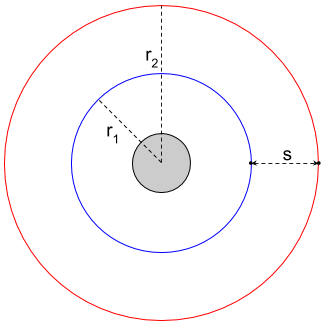
\includegraphics[width=0.3\textwidth]{schwarz.png}
		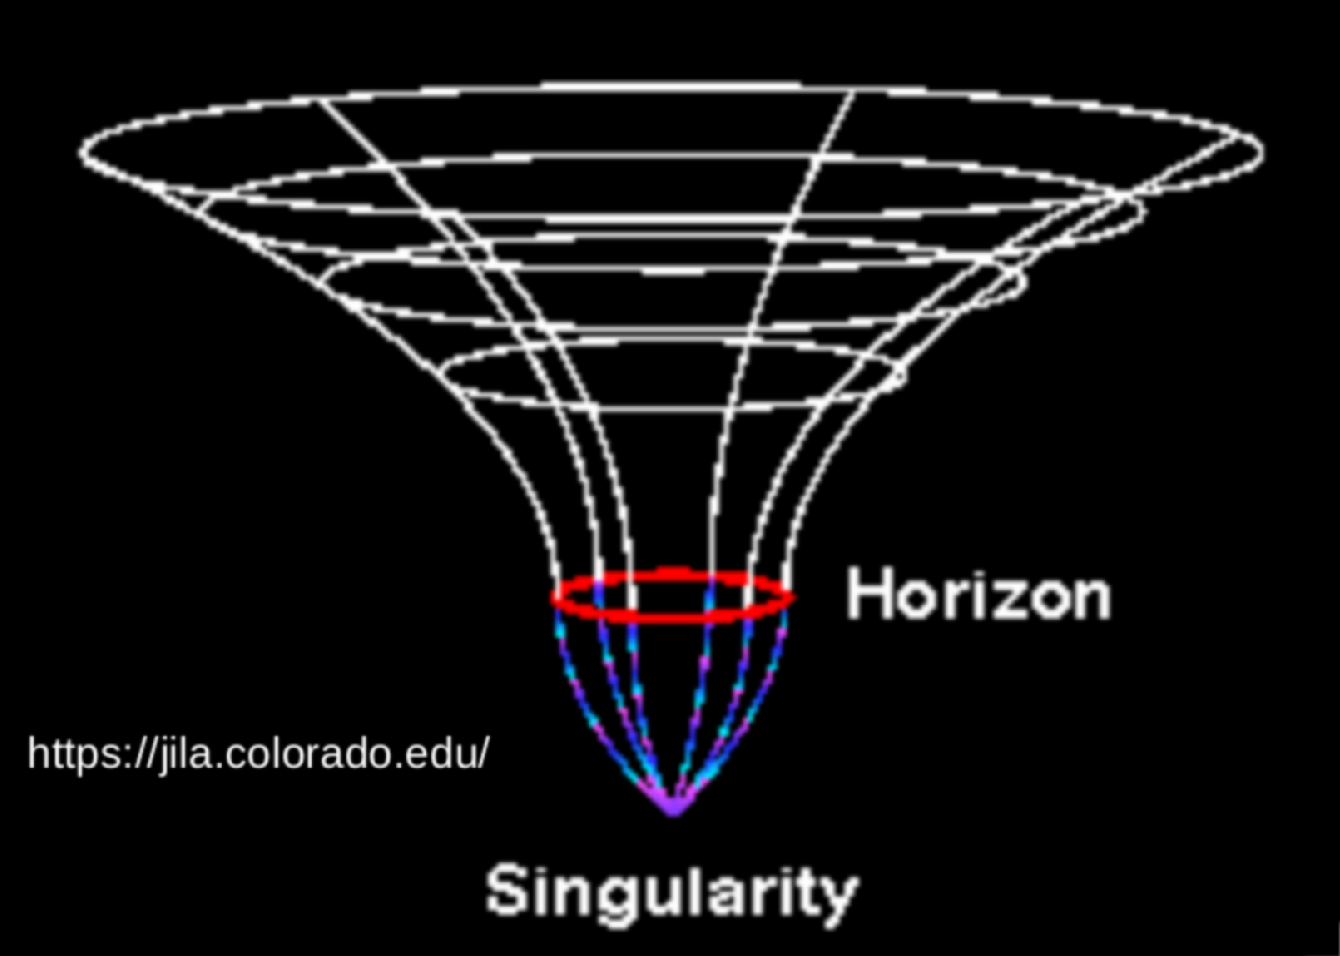
\includegraphics[width=0.4\textwidth]{blackhole.png}
	\end{figure}
	
	Berbeda dengan \textit{proper time}, untuk menghitung \textit{proper distance} perlu dilakukan integrasi. Untuk kasus $d\theta = d\varphi = 0$
	\begin{eqnarray*}
	ds &=& \frac{dr}{\sqrt{1 - \frac{r_s}{r}}}\\
	s &=& \int_{r_1}^{r_2} \frac{dr}{\sqrt{1 - \frac{r_s}{r}}}\\
	s &=& \left[ r \sqrt{1 - \frac{r_s}{r}} + \frac{1}{2} r_s \ln{\left( 2r \left( \sqrt{1 - \frac{r_s}{r}} + 1 \right) - r_s \right)} \right]_{r_1}^{r_2}
	\end{eqnarray*}

	\begin{itemize}
		\item jarak proper dari $r=10$ km ke $r=20$ km, s = 11,3545 km
		\item jarak proper dari $r=10$ km ke $r=30$ km, s = 22,0773 km
	\end{itemize}
	
	\vspace{0.5cm}
	\textit{Catatan:} \\
	Apakah yang dimaksud soal bukan jarak proper? \textit{null geodesic}?
	
	
\end{enumerate}




\end{questions}

%\centering{\--- SOAL SELESAI\---}

\vspace{3cm}
\begin{flushright}
Hitungan lebih detail bisa di cek di \url{https://s.id/HitunganOSP2019}\\
Solusi seperti ini dapat diperoleh di \url{http://ridlow.wordpress.com}
\end{flushright}
\end{document}
